\documentclass[twocolumn]{phdsymp} %!PN
\usepackage[english]{babel}

\usepackage{graphicx}                   % Om figuren te kunnen verwerken
\usepackage{graphics}					% Om figuren te verwerken.
\graphicspath{{figuren/}}               % De plaats waar latex zijn figuren gaat halen.

\usepackage{times}

\hyphenation{}

\def\BibTeX{{\rm B\kern-.05em{\sc i\kern-.025em b}\kern-.08em
    T\kern-.1667em\lower.7ex\hbox{E}\kern-.125emX}}

\newtheorem{theorem}{Theorem}

\begin{document}

\title{Realtime signal synchronization with accoustic fingerprinting} %!PN

\author{Ward Van Assche}

\supervisor{Joren Six, Marleen Denert}

\maketitle

\begin{abstract}
Sed nec tortor in libero rutrum pellentesque et gravida turpis. Phasellus gravida neque vitae elit fringilla, a efficitur purus sollicitudin. Proin lacus est, suscipit sed nibh ac, hendrerit eleifend leo. Suspendisse quis semper leo. Duis non elit commodo, sodales ex non, venenatis diam. Sed libero tortor, hendrerit et sollicitudin ut, facilisis vitae odio. Fusce vitae mi odio.
\end{abstract}

\begin{keywords}
kernwoord1, kernwoord2, kernwoord 3, kernwoord 4
\end{keywords}

\section{Introduction}
\PARstart{S}{ed} Sed nec tortor in libero rutrum pellentesque et gravida turpis. Phasellus gravida neque vitae elit fringilla, a efficitur purus sollicitudin. Proin lacus est, suscipit sed nibh ac, hendrerit eleifend leo. Suspendisse quis semper leo. Duis non elit commodo, sodales ex non, venenatis diam. Sed libero tortor, hendrerit et sollicitudin ut, facilisis vitae odio. Fusce vitae mi odio. Cras vitae quam bibendum, elementum velit ut, varius enim. Donec sagittis elit ligula, laoreet viverra felis rhoncus nec. Donec mattis metus pretium, pulvinar enim a, luctus nunc. Pellentesque quis suscipit leo.


\section{Sectie}

\subsection{Subsectie}
Sed nec tortor in libero rutrum pellentesque\cite{six2014tarsosdsp} et gravida turpis. Phasellus gravida neque vitae elit fringilla, a efficitur purus sollicitudin. Proin lacus est, suscipit sed nibh ac, hendrerit eleifend leo. Suspendisse quis semper leo. Duis non elit commodo, sodales ex non, venenatis diam. Sed libero tortor, hendrerit et sollicitudin ut, facilisis vitae odio. Fusce vitae mi odio. Cras vitae quam bibendum, elementum velit ut, varius enim. Donec sagittis elit ligula, laoreet viverra felis rhoncus nec. Donec mattis metus pretium, pulvinar enim a, luctus nunc. Pellentesque quis suscipit leo.

\subsection{Andere subsectie}
Sed nec tortor in libero rutrum pellentesque et gravida turpis. Phasellus gravida neque vitae elit fringilla, a efficitur purus sollicitudin. Proin lacus est, suscipit sed nibh ac, hendrerit eleifend leo. Suspendisse quis semper leo. Duis non elit commodo, sodales ex non, venenatis diam. Sed libero tortor, hendrerit et sollicitudin ut, facilisis vitae odio. Fusce vitae mi odio. Cras vitae quam bibendum, elementum velit ut, varius enim. Donec sagittis elit ligula, laoreet viverra felis rhoncus nec. Donec mattis metus pretium, pulvinar enim a, luctus nunc. Pellentesque quis suscipit leo.

Sed nec tortor in libero rutrum pellentesque et gravida turpis. Phasellus gravida neque vitae elit fringilla, a efficitur purus sollicitudin. Proin lacus est, suscipit sed nibh ac, hendrerit eleifend leo. Suspendisse quis semper leo. Duis non elit commodo, sodales ex non, venenatis diam. Sed libero tortor, hendrerit et sollicitudin ut, facilisis vitae odio. Fusce vitae mi odio. Cras vitae quam bibendum, elementum velit ut, varius enim. Donec sagittis elit ligula, laoreet viverra felis rhoncus nec. Donec mattis metus pretium, \textit{pulvinar} enim a, luctus nunc. Pellentesque quis suscipit leo.

\begin{figure}[ht]
	\begin{center}
		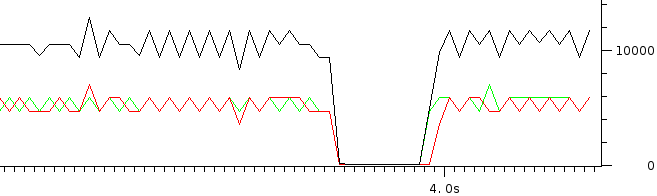
\includegraphics[width=.40\textwidth]{referentie-detail}
		\caption{\label{2AP}Detailed capture of the stream at the moment of a handover between two simulated AP's with a strong signal.  Notice the gap of 100~ms.}
	\end{center}
\end{figure}

\section{Sectie}
Aenean auctor congue nisi, volutpat porta urna lobortis in. Donec accumsan fermentum lectus, sed aliquet lectus gravida eget. Ut turpis quam, fermentum eget sem sed, euismod facilisis sem. Etiam a sollicitudin purus. Vestibulum quis nisl et nibh condimentum suscipit tristique eget quam. Aenean eget varius lectus. Maecenas sit amet mi augue. Nullam semper ex et facilisis ullamcorper. Cras volutpat ornare arcu, ac suscipit nisi pellentesque iaculis. Vivamus sit amet ipsum consequat, egestas massa varius, aliquam lorem. Aenean ornare iaculis dolor, eget efficitur elit. Maecenas ut massa ac tortor hendrerit pulvinar a in ante.

\section{Conclusion}
The simulation results show a nice advantage for the moving² cell\cite{six2015multimodal} concept.  The traditional handover problem can be avoided so a workable model for broadband access on trains seems realistic.  But there needs to be done a lot of research to make RAU's and RoF as reliable and cheap as possible.

\bibliographystyle{phdsymp}
\bibliography{../bronnen/bronnen}

\end{document}

%%%%%%%%%%%%%%%%%%%%%  End of phdsymp_sample2e.tex  %%%%%%%%%%%%%%%%%%%%%%%%%%%
